%\documentclass[a4paper,superscriptaddress,11pt]{quantumarticle}
%\documentclass[aps,twocolumn,longbibliography,english,superscriptaddress]{revtex4-1}
\documentclass{article}
\usepackage{iclr2021_conference}
%\documentclass[a4paper,superscriptaddress,11pt]{article}
\pdfoutput=1
\usepackage[colorlinks=true,urlcolor=blue,citecolor=blue,linkcolor=blue]{hyperref}
\usepackage[english]{babel}
\usepackage[utf8]{inputenc}
\usepackage[T1]{fontenc}
\usepackage{amssymb}
\usepackage{tabularx}
\usepackage{quoting}
\usepackage{upquote}
\usepackage{subcaption}
\usepackage{multicol}
\usepackage[framemethod=TikZ]{mdframed}
\usepackage{wrapfig}
%\usepackage{caption}
%\usepackage[plain]{algorithm}
\usepackage[ruled, vlined]{algorithm2e}
\usepackage{algpseudocode}
\usepackage{rotating}
%\usepackage{cite}
\usepackage{booktabs}
%\usepackage{unicode-math}
%\usepackage{algorithm}% http://ctan.org/pkg/algorithm
%\usepackage{algpseudocode}% http://ctan.org/pkg/algpseudocode
\usepackage{xcolor}% http://ctan.org/pkg/xcolor
\makeatletter
\newsavebox{\@brx}
\newcommand{\llangle}[1][]{\savebox{\@brx}{\(\m@th{#1\langle}\)}%
  \mathopen{\copy\@brx\kern-0.5\wd\@brx\usebox{\@brx}}}
\newcommand{\rrangle}[1][]{\savebox{\@brx}{\(\m@th{#1\rangle}\)}%
  \mathclose{\copy\@brx\kern-0.5\wd\@brx\usebox{\@brx}}}
\makeatother
\usepackage{bbm}
\usepackage{jlcode}
\usepackage{graphicx}
\usepackage{amsmath,color,amsthm}
\usepackage{mathrsfs}
\usepackage{float}
\usepackage[normalem]{ulem}
\usepackage{indentfirst}
\usepackage{txfonts}
\usepackage[epsilon, tsrm, altpo]{backnaur}

\newcommand{\listingcaption}[1]%
{%
\refstepcounter{lstlisting}\hfill%
Listing \thelstlisting: #1\hfill%\hfill%
}%
\newcolumntype{b}{X}
\newcolumntype{s}{>{\hsize=.7\hsize}X}
\usepackage{listings}
\lstset{
    language=Julia,
    basicstyle=\ttfamily\scriptsize,
    numberstyle=\scriptsize,
    % numbers=left,
    backgroundcolor=\color{gray!7},
    %backgroundcolor=\color{white},
    %frame=single,
    xleftmargin=2em,
    tabsize=2,
    rulecolor=\color{black!15},
    %title=\lstname,
    escapeinside={(*}{*)},
    breaklines=true,
    %breakatwhitespace=true,
    %framextopmargin=2pt,
    %framexbottommargin=2pt,
    frame=bt,
    extendedchars=true,
    inputencoding=utf8,
    columns=fullflexible,
    %escapeinside={(*@}{@*)},
}

\tolerance=1
\emergencystretch=\maxdimen
\hyphenpenalty=1000
\hbadness=1000

\makeatletter

%%%%%%%%%%%%%%%%%%%%%%%%%%%%%% User specified LaTeX commands.

%Journal reference.  Comma sets off: name, vol, page, year
\def\journal #1, #2, #3, 1#4#5#6{{\sl #1~}{\bf #2}, #3 (1#4#5#6) }
\def\pr{\journal Phys. Rev., }
\def\prb{\journal Phys. Rev. B, }
\def\prl{\journal Phys. Rev. Lett., }
\def\pl{\journal Phys. Lett., }
%\def\np{\journal Nucl. Phys., }


%%%%%%%%%%%%%%%%%%%%%%%%%%%%%%%%%%%%%%%%%%%%%%%%%%%%%%%%%%%%%%%%%%%%%%%%%%%%%%%%%%%%%%%%%%%%%%%%%%%%%%%%%%%%%%%%%%%%%%%%%%%%%%%%%%%%%%%%%%%%%%%%%%%%%%%%%%%%%%%%%%%%%%%%%%%%%%%%%%%%%%%%%%%%%%%%%%%%%%%%%%%%%%%%%%%%%%%%%%%%%%%%%%%%%%%%%%%%%%%%%%%%%%%%%%%%


%\usepackage{CJK}
%\usepackage[colorlinks, citecolor=blue]{hyperref}
\DeclareMathOperator*{\argmax}{arg\,max}

%%%%%% Shortcut related
\newcommand{\<}{\langle}
\renewcommand{\>}{\rangle}
\newcommand{\out}{{\vx^L}}
\newcommand{\inp}{{\vx^0}}
\newcommand{\cquad}{{{ }_{\quad}}}
\newcommand{\pluseq}{\mathrel{+}=}
\newcommand{\minuseq}{\mathrel{-}=}
\newcommand{\vx}{{\mathbf{x}}}
\newcommand{\vg}{{\mathbf{g}}}
\newcommand{\vp}{{\mathbf{p}}}
\newcommand{\vy}{{\mathbf{y}}}
\newcommand{\Var}{{\mathrm{Var}}}
\newcommand{\Mean}{{\mathrm{E}}}
\newcommand{\vvalue}{{\texttt{value}}}
\newcommand{\grad}{{\texttt{grad}}}
\newcommand{\parameter}{{\texttt{parameter}}}
%%%%%% Convention related
\newcommand{\SWAP}{{\rm SWAP}}
\newcommand{\CNOT}{{\rm CNOT}}
\newcommand{\X}{{\rm X}}
\renewcommand{\H}{{\rm H}}
\newcommand{\Rx}{{\rm Rx}}
\renewcommand{\v}[1]{{\bf #1}}
\newcommand{\dataset}{{\mathcal{D}}}
\newcommand{\wfunc}{{\psi}}
\newcommand{\SU}{{\rm SU}}
\newcommand{\UU}{{\rm U}}
\newcommand{\thetav}{{\boldsymbol{\theta}}}
\newcommand{\gammav}{{\boldsymbol{\gamma}}}
\newcommand{\thetai}{{\theta^\alpha_l}}
\newcommand{\Expect}{{\mathbb{E}}}
\newcommand{\Tr}{{\rm Tr}}
\newcommand{\etc}{{\it etc~}}
\newcommand{\etal}{{\it etal~}}
\newcommand{\xset}{\mathbf{X}}
\newcommand{\fl}{\texttt{fl}}
\newcommand{\pdata}{\mathbf{\pi}}
\newcommand{\q}{\mathbf{q}}
\newcommand{\epdata}{\mathbf{\hat{\pi}}}
\newcommand{\gammaset}{\boldsymbol{\Gamma}}
\newcommand{\ei}{{\mathbf{e}_l^\alpha}}
\newcommand{\vtheta}{{\boldsymbol{\theta}}}
\newcommand{\sigmag}{{\nu}}
\newcommand{\sigmai}[2]{{\sigma^{#2}_{#1}}}
\newcommand{\qi}[1]{{q^{\alpha_{#1}}_{#1}}}
\newcommand{\BAS}{Bars-and-Stripes}
\newcommand{\circled}[1]{\raisebox{.5pt}{\textcircled{\raisebox{-.9pt} {#1}}}}

\newcommand{\qexpect}[1]{{\left\langle #1\right\rangle}}
\newcommand{\expect}[2]{{\mathop{\mathbb{E}}\limits_{\substack{#2}}\left[#1\right]}}
\newcommand{\var}[2]{{\mathop{\mathrm{Var}}\limits_{\substack{#2}}\left(#1\right)}}
\newcommand{\pshift}[1]{{p_{\thetav+#1}}}
\newcommand{\upcite}[1]{\textsuperscript{\cite{#1}}}
\newcommand{\Eq}[1]{Eq.~(\ref{#1})}
\newcommand{\Fig}[1]{Fig.~\ref{#1}}
\newcommand{\Lst}[1]{Listing.~\ref{#1}}
\newcommand{\Tbl}[1]{Table~\ref{#1}}
\newcommand{\Sec}[1]{Sec.~\ref{#1}}
\newcommand{\App}[1]{Appendix~\ref{#1}}
\newcommand{\bra}[1]{\mbox{$\left\langle #1 \right|$}}
\newcommand{\ket}[1]{\mbox{$\left| #1 \right\rangle$}}
\newcommand{\braket}[2]{\mbox{$\left\langle #1 | #2 \right\rangle$}}
\newcommand{\tr}[1]{\mathrm{tr}\mbox{$\left[ #1\right]$}}

\newcommand{\ra}[1]{\renewcommand{\arraystretch}{#1}}

%%%%%% Comment related
\newcommand{\red}[1]{[{\bf  \color{red}{LW: #1}}]}
\newcommand{\xred}[1]{[{\bf  \color{red}{\sout{LW: #1}}}]}
\newcommand{\blue}[1]{[{\bf  \color{blue}{JG: #1}}]}
\newcommand{\violet}[1]{[{\bf  \color{violet}{MLS: #1}}]}
\newcommand{\green}[1]{[{\bf  \color{green}{TZ: #1}}]}
\newcommand{\xgreen}[1]{[{\bf  \color{green}{\sout{TZ: #1}}}]}
\newcommand{\xblue}[1]{[{\bf  \color{blue}{\sout{JG: #1}}}]}
\newcommand{\material}[1]{\iffalse[{\bf  \color{cyan}{Material: #1}}]\fi}
\newcommand{\orange}[1]{\iffalse[{\bf  \color{orange}{Jo: #1}}]\fi}

\newtheorem{theorem}{\textit{Theorem}}
\theoremstyle{definition}\newtheorem{definition}{\textit{Definition}}

\makeatother

\begin{document}
\title{Differentiate Everything with a Reversible Embeded Domain-Specific Language}

\author{Jin-Guo Liu\\
Institute of Physics, Chinese Academy of Sciences,\\Beijing 100190, China\\
\texttt{cacate0129@iphy.ac.cn}\\
\And
Taine Zhao\\
Department of Computer Science, University of Tsukuba\\
\texttt{thaut@logic.cs.tsukuba.ac.jp}\\
}
\maketitle

\begin{abstract}
Reverse-mode automatic differentiation (AD) suffers from the issue of having too much space overhead to trace back intermediate computational states for back-propagation.
The traditional method to trace back states is called checkpointing that stores intermediate states into a global stack and restore state through either stack pop or re-computing.
The overhead of stack manipulations and re-computing makes the general purposed (not tensor-based) AD engines unable to meet many industrial needs.
Instead of checkpointing, we propose to use reverse computing to trace back states by designing and implementing a reversible programming eDSL, where a program can be executed bi-directionally without implicit stack operations. The absence of implicit stack operations makes the program compatible with existing compiler features, including utilizing existing optimization passes and compiling the code as GPU kernels.
We implement AD for sparse matrix operations and some machine learning applications to show that the performance of our framework has state-of-the-art performance.
\end{abstract}

\section{Introduction}\label{sec:intro}
  Most of the popular automatic differentiation (AD) tools in the market, such as TensorFlow~\cite{Tensorflow2015}, Pytorch~\cite{Paszke2017}, and Flux~\cite{Innes2018a} implements reverse mode AD at the tensor level to meet the need in machine learning. Later, People in the scientific computing domain also realized the power of these AD tools, they use these tools to solve scientific problems such as seismic inversion~\cite{Zhu2020}, variational quantum circuits simulation~\cite{Bergholm2018} and variational tensor network simulation~\cite{Liao2019,Roberts2019}. To meet the diverse need in these applications, one sometimes has to define backward rules manually, for example
\begin{enumerate}
\item To differentiate sparse matrix operations used in Hamiltonian engineering~\cite{Xie2020}, people defined backward rules for sparse matrix multiplication and dominant eigensolvers~\cite{Golub2012},
\item In tensor network algorithms to study the phase transition problem~\cite{Liao2019,Seeger2017,Wan2019,Hubig2019}, people defined backward rules for singular value decomposition (SVD) function and QR decomposition~\cite{Golub2012}.
\end{enumerate}
To avoid defining backward rules manually, one can also use a general purposed AD (GP-AD) software like Tapenade~\cite{Hascoet2013}, OpenAD~\cite{Utke2008} and Zygote~\cite{Innes2018, Innes2019} to differentiate a general program. These tools have been used in non-tensor based applications such as bundle adjustment~\cite{Shen2018} and earth system simulation~\cite{Forget2015}.
However, these tools have their limitations too. In many practical applications, differentiating a program might do billions of computations. Frequent caching of data slows down the program significantly, while the memory usage will become a bottleneck as well. Although most of them are source-code-transformation based, they can not be used to differentiate GPU kernel functions because implicit stack operations are not compatible with kernel functions.

We need a new GP-AD framework that does not cache for users automatically. Hence we propose to implement the reverse mode AD on a reversible (domain-specific) programming language~\cite{Perumalla2013,Frank2017}, where intermediate states can be traced backward without accessing an implicit stack.
Reversible programming provides flexible time-space trade-off.
It also allows people to utilize the reversibility to reverse a program without any overhead.
In machine learning, reversibility is proven to significantly decrease the memory usage in unitary recurrent neural networks~\cite{MacKay2018}, normalizing flow~\cite{Dinh2014}, hyper-parameter learning~\cite{Maclaurin2015} and residual neural networks~\cite{Behrmann2018}.
Reversible programming will make these happen naturally.

There have been many prototypes of reversible languages like Janus~\cite{Lutz1986}, R (not the popular one)~\cite{Frank1997}, Erlang~\cite{Lanese2018} and object-oriented ROOPL~\cite{Haulund2017}.
In the past, the primary motivation to study reversible programming is to support reversible computing devices~\cite{Frank1999} such as adiabatic complementary metal-oxide-semiconductor (CMOS)~\cite{Koller1992}, molecular mechanical computing system~\cite{Merkle2018} and superconducting system~\cite{Likharev1977,Semenov2003,Takeuchi2014,Takeuchi2017}, and these reversible computing devices are orders more energy-efficient. Landauer~\cite{Landauer1961} proves that only when a device does not erase information (i.e. reversible), its energy efficiency can go beyond the thermal dynamic limit.
However, these reversible programming languages can not be used in real scientific computing, since most of them do not have basic elements like floating point numbers, arrays, and complex numbers. This motivates us to build a new embedded domain-specific language (eDSL) in Julia~\cite{Bezanson2012,Bezanson2017} as a new playground of GP-AD.

    In this paper, we first introduce the language design of NiLang in \Sec{sec:lang}.
    In \Sec{sec:bp}, we explain the implementation of automatic differentiation in NiLang.
    In \Sec{sec:benchmark}, we benchmark the performance of NiLang's AD with other AD software and explain why it is fast.

\section{Language design}\label{sec:lang}

NiLang is an embedded domain-specific language (eDSL) NiLang on top of the host language Julia~\cite{Bezanson2012,Bezanson2017}.
Julia is a popular language for scientific programming and machine learning. We choose Julia mainly for speed. Julia is a language with high abstraction, however, its clever design of type inference and just in time compiling make it has a C like speed.
Meanwhile, it has rich features for meta-programming. Its package for pattern matching \href{https://github.com/thautwarm/MLStyle.jl}{MLStyle} allows us to define an eDSL in less than 2000 lines.
Comparing with a regular reversible programming language, NiLang features array operations, rich number systems including floating-point numbers, complex numbers, fixed-point numbers, and logarithmic numbers.
It also implements the compute-copy-uncompute~\cite{Bennett1973} macro to increase code reusability.
Besides the above ``nice'' features, it also has some ``bad'' features to meet the practical needs. For example, it views the floating-point $\mathrel{+}$ and $\mathrel{-}$ operations as reversible. It also allows users to extend instruction sets and sometimes inserting external statements. These features are not compatible with future reversible hardware.
NiLang's source code is available online \href{https://github.com/GiggleLiu/NiLang.jl}{https://github.com/GiggleLiu/NiLang.jl}, \href{https://github.com/GiggleLiu/NiLangCore.jl}{https://github.com/GiggleLiu/NiLangCore.jl}.
By the time of writing, the version of NiLang is v0.7.2.

\subsection{Reversible functions and instructions}
    Mathematically, any irreversilbe mapping \texttt{y = f(args...)} can be trivially transformed to its reversible form \texttt{y += f(args...)} or \texttt{y $\veebar$= f(args...)} ($\veebar$ is the bit-wise \texttt{XOR}), where \texttt{y} is a pre-emptied variable. But in numeric computing with finite precision, this is not always true. The reversibility of arithmetic instruction is closely related to the number system.
    For integer and fixed point number system, \texttt{y += f(args...)} and \texttt{y -= f(args...)} are rigorously reversible. For logarithmic number system and tropical number system~\cite{Speyer2009}, \texttt{y *= f(args...)} and \texttt{y /= f(args...)} as reversible (not introducing the zero element). While for floating point numbers, none of the above operations are regorously reversible. However, for convenience, we ignore the rounding errors in floating point \texttt{+} and \texttt{-} operations and treat them on equal footing with fixed point numbers in the following discussion.
Other reversible operations includes \texttt{SWAP}, \texttt{ROT}, \texttt{NEG} et. al., and this instruction set is extensible.

The following code defines a reversible multiplier.

\begin{minipage}{.88\columnwidth}
\begin{lstlisting}[mathescape=true,caption={A reversible multiplier},label={lst:multiplier}]
julia> using NiLang

julia> @i function multiplier(y!::Real, a::Real, b::Real)
           y! += a * b
       end

julia> multiplier(2, 3, 5)
(17, 3, 5)

julia> (~multiplier)(17, 3, 5)
(2, 3, 5)
\end{lstlisting}
\end{minipage}

Macro \texttt{@i} generates two functions that are reversible to each other, \texttt{multiplier} and \texttt{$\sim$multiplier}, each defines a mapping $\mathbb{R}^3 \rightarrow \mathbb{R}^3$. The $!$ after a symbol is a part of the name, as a conversion to indicate the mutated variables.

\subsection{Reversible memory management}
    A distinct feature of reversible memory management is that the content of a variable must be known when it is deallocated.
    We denote the allocation of a pre-emptied memory as \texttt{x $\leftarrow$ 0}, and its inverse, deallocating a \textbf{zero emptied} variable, as \texttt{x $\rightarrow$ 0}.
    An unknown variable can be pushed to a stack and used in the uncomputing stage with a pop statement.
    If a variable is allocated and deallocated in the local scope, we call it an ancilla.

\begin{minipage}{.45\columnwidth}
\begin{lstlisting}[mathescape=true,caption={Reversible complex valued log function $y\mathrel{+}=\log(|x|) + i{\rm Arg}(x)$.},label={lst:complex}]
@i @inline function (:+=)(log)(y!::Complex{T}, x::Complex{T}) where T
    n ← zero(T)
    n += abs(x)

    y!.re += log(n)
    y!.im += angle(x)

    n -= abs(x)
    n → zero(T)
end
\end{lstlisting}
\end{minipage}\hfill
\begin{minipage}{.45\columnwidth}
    \begin{lstlisting}[mathescape=true,caption={Compute-copy-uncompute version of \Lst{lst:complex}},label={lst:complex2}]
@i @inline function (:+=)(log)(y!::Complex{T}, x::Complex{T}) where T
    @routine begin
        n ← zero(T)
        n += abs(x)
    end
    y!.re += log(n)
    y!.im += angle(x)
    ~@routine
end
\end{lstlisting}
\end{minipage}

\Lst{lst:complex} defines the complex valued accumulative log function.
The macro \texttt{@inline} tells the compiler that this function can be inlined. One can input ``$\leftarrow$'' and ``$\rightarrow$'' by typing ``$\backslash$leftarrow[TAB KEY]'' and ``$\backslash$rightarrow[TAB KEY]'' respectively in a Julia editor or REPL.
NiLang does not have immutable structs, so that the real part \texttt{y!.re} and imaginary \texttt{y!.im} of a complex number can be changed directly.
It is easy to verify that the bottom two lines in the function body are the inverse of the top two lines. i.e., the bottom two lines \textit{uncomputes} the top two lines.
The motivation of uncomputing is to zero clear the contents in ancilla \texttt{n} so that it can be deallocated correctly.
\textit{Compute-copy-uncompute} is a useful design pattern in reversible programming so that we created a pair of macros \texttt{@routine} and \texttt{$\sim$@routine} for it. One can rewrite the above function as in \Lst{lst:complex2}.

\subsection{Reversible control flows}
One can define reversible \texttt{if}, \texttt{for} and \texttt{while} statements in a reversible program.
\Fig{fig:controlflow} (a) shows the flow chart of executing the reversible \texttt{if} statement. There are two condition expressions in this chart, a precondition and a postcondition. The precondition decides which branch to enter in the forward execution. After executing the specific branch, the program checks the consistency between precondition and postcondition to make sure they are consistent. To reverse this statement, one can exchange the precondition and postcondition, and reverse the expressions in both branches.
\Fig{fig:controlflow} (b) shows the flow chart of the reversible \texttt{while} statement. There are also two conditions expressions. Before executing the condition expressions, the program presumes the postcondition is false.
After each iteration, the program asserts the postcondition to be true. To reverse this statement, one can exchange the precondition and postcondition, and reverse the body statements.
The reversible \texttt{for} statement is similar to the irreversible one except that after execution, the program will assert the iterator to be unchanged. To reverse this statement, one can exchange \texttt{start} and \texttt{stop} and inverse the sign of \texttt{step}.
\begin{figure}
    \centerline{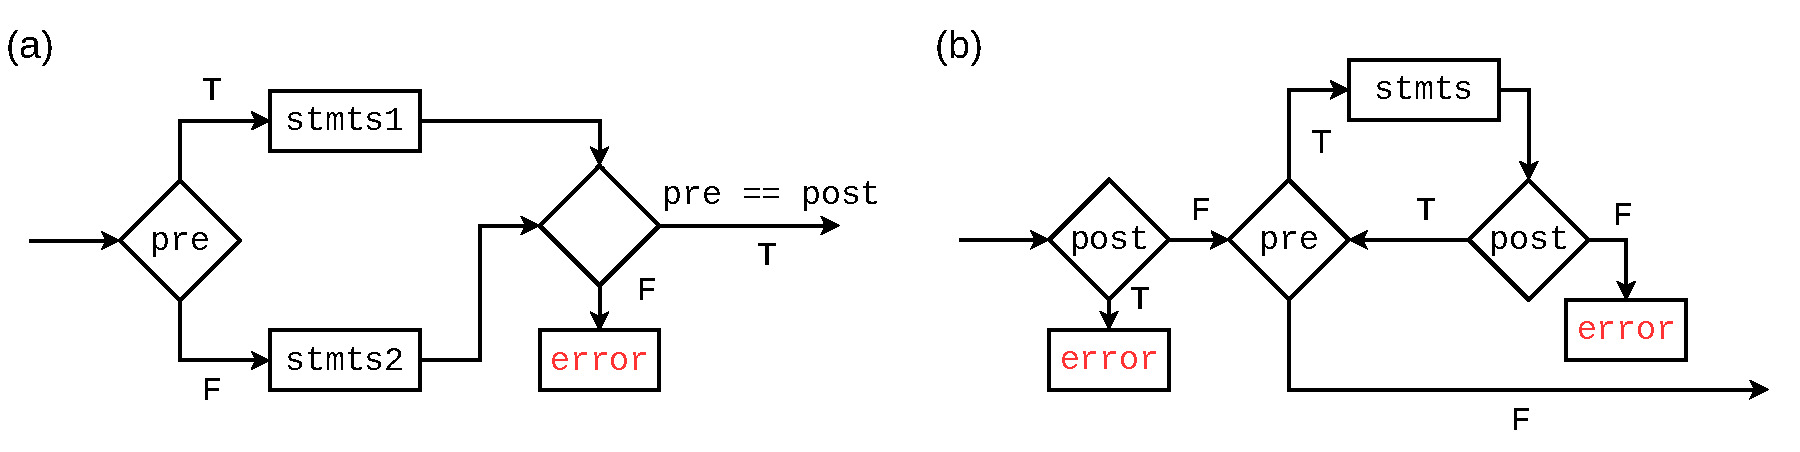
\includegraphics[width=0.9\columnwidth,trim={0 0cm 0 0cm},clip]{controlflow_v2.pdf}}
    \caption{The flow chart for reversible (a) \texttt{if} statement and (b) \texttt{while} statement. ``pre'' and ``post'' represents precondition and postcondition respectively.}\label{fig:controlflow}
\end{figure}

The following code computes the Fibonacci number recursively and reversibly.

\begin{minipage}{.88\columnwidth}
\begin{lstlisting}[mathescape=true,caption={Computing Fibonacci number recursively and reversibly.},label={lst:fib}]
@i function rrfib(out!, n)
    @invcheckoff if (n >= 1, ~)
        counter ← 0
        counter += n
        while (counter > 1, counter!=n)
            rrfib(out!, counter-1)
            counter -= 2
        end
        counter -= n % 2
        counter → 0
    end
    out! += 1
end
\end{lstlisting}
\end{minipage}

Here, \texttt{out!} is an integer initialized to \texttt{0} for storing outputs.
The precondition and postcondition are wrapped into a tuple. In the \texttt{if} statement, the postcondition is the same as the precondition, hence we omit the postcondition by inserting a "\texttt{$\sim$}" in the second field as a placeholder.
In the while statement, the postcondition is true only for the initial loop.
Once code is proven correct, one can turn off the reversibility check by adding \texttt{@invcheckoff} before a statement.
This will remove the reversibility check and make the code faster and compatible with GPU kernels (kernel functions can not handle exceptions).

\subsection{Reverse computing is not checkpointing}\label{sec:timespace}
There are two approaches to trace back intermediate states of a computational process, one is checkpointing~\cite{Griewank2008, Chen2016} and another is reverse computing.
Reverse computing and checkpointing share many similarities.
When there is no time overhead, both have a space overhead $\sim O(T)$ (i.e. linear to time).
They also have many differences. When a polynomial overhead in time is allowed, reversible computing has a minimum space overhead of $O(S\log(T))$~\cite{Bennett1989,Levine1990,Perumalla2013}.
For checkpointing, there can be no space overhead, since one can just recompute from beginning to obtain any intermediate state with time complexity $O(T^2)$.
In practical using cases, reverse computing has the following advantages.

Reverse computing shows the advantage of handling effective codes with mutable structures and arrays.
For example, the affine transformation can be implemented without any overhead.

\begin{minipage}{.88\columnwidth}
\begin{lstlisting}[mathescape=true,caption={Inplace affine transformation.},label={lst:affine}]
@i function i_affine!(y!::AbstractVector{T}, W::AbstractMatrix{T}, b::AbstractVector{T}, x::AbstractVector{T}) where T
    @safe @assert size(W) == (length(y!), length(x)) && length(b) == length(y!)
    @invcheckoff for j=1:size(W, 2)
        for i=1:size(W, 1)
            @inbounds y![i] += W[i,j]*x[j]
        end
    end
    @invcheckoff for i=1:size(W, 1)
        @inbounds y![i] += b[i]
    end
end
\end{lstlisting}
\end{minipage}

Here, the expression following the \texttt{@safe} macro is an external irreversible statement.

Reverse computing can utilize reversibility to trace back states without extra memory cost.
For example, we can define the unitary matrix multiplication that can be used in a type of memory-efficient recurrent neural network~\cite{Jing2016}.

\begin{minipage}{.88\columnwidth}
\begin{lstlisting}[mathescape=true,caption={Two level decomposition of a unitary matrix.},label={lst:affine}]
@i function i_umm!(x!::AbstractArray, θ)
    M ← size(x!, 1)
    N ← size(x!, 2)
    k ← 0
    @safe @assert length(θ) == M*(M-1)/2
    for l = 1:N
        for j=1:M
            for i=M-1:-1:j
                INC(k)
                ROT(x![i,l], x![i+1,l], θ[k])
            end
        end
    end
    k → length(θ)
end
\end{lstlisting}
\end{minipage}

Last but not least, reversible programming encourages users to code in a memory friendly style.
Since allocations in reversible programming are explicit, programmers have the flexibility to control how to allocate memory and which number system to use.
For example, to compute the power of a positive fixed-point number and an integer, one can easily write irreversible code as in \Lst{lst:power1}

\begin{minipage}{.45\columnwidth}
\begin{lstlisting}[mathescape=true,caption={A regular power function.},label={lst:power1}]
function mypower(x::T, n::Int) where T
    y = one(T)
    for i=1:n
        y *= x
    end
    return y
end
\end{lstlisting}
\end{minipage}\hfill
\begin{minipage}{.45\columnwidth}
\begin{lstlisting}[mathescape=true,caption={A reversible power function.},label={lst:power2}]
@i function mypower(out,x::T,n::Int) where T
    if (x != 0, ~)
        @routine begin
            ly ← one(ULogarithmic{T})
            lx ← one(ULogarithmic{T})
            lx *= convert(x)
            for i=1:n
                ly *= x
            end
        end
        out += convert(ly)
        ~@routine
    end
end
\end{lstlisting}
\end{minipage}

Since the fixed-point number is not reversible under \texttt{*=}, naive checkpointing would require stack operations inside a loop. With reversible thinking, we can convert the fixed-point number to logarithmic numbers to utilize the reversibility of \texttt{*=} as shown in \Lst{lst:power2}. Here, the algorithm to convert a regular fixed-point number to a logarithmic number can be efficient~\cite{Turner2010}.

\section{Reversible automatic differentiation}\label{sec:bp}

\subsection{Backpropagation}\label{sec:jacobian}
To backpropagate the program, we first reverse the code through source code transformation and then insert the gradient code through operator overloading.
If we inline all the instructions in \Lst{lst:complex2}, the program would be like \Lst{lst:expand-complex}.
The automatically generated inverse program (i.e. $(y, x) \rightarrow (y-\log(x), x)$) is like \Lst{lst:reversed-complex}.

\begin{minipage}{.45\textwidth}
\begin{lstlisting}[mathescape=true,caption={The function body of \Lst{lst:complex2}.},label={lst:expand-complex}, frame=tlrb]
@routine begin
    nsq ← zero(T)
    n ← zero(T)
    nsq += x[i].re ^ 2
    nsq += x[i].im ^ 2
    n += sqrt(nsq)
end
y![i].re += log(n)
y![i].im += atan(x[i].im, x[i].re)
~@routine
\end{lstlisting}
\end{minipage}\hfill
\begin{minipage}{.45\textwidth}
    \begin{lstlisting}[mathescape=true,caption={The inverse of \Lst{lst:expand-complex}.},label={lst:reversed-complex}, frame=tlrb]
@routine begin
    nsq ← zero(T)
    n ← zero(T)
    nsq += x[i].re ^ 2
    nsq += x[i].im ^ 2
    n += sqrt(nsq)
end
y![i].re -= log(n)
y![i].im -= atan(x[i].im, x[i].re)
~@routine
\end{lstlisting}
\end{minipage}

To compute the adjoint of the computational process in \Lst{lst:expand-complex}, one simply insert the gradient code into its inverse in \Lst{lst:reversed-complex}.
The resulting inlined code is show in \Lst{lst:grad-complex}.

\begin{minipage}{.88\columnwidth}
\listingcaption{Insert the gradient code into \Lst{lst:reversed-complex}, the original computational processes are highlighted in yellow background.}\label{lst:grad-complex}
\begin{lstlisting}[mathescape=true,label={lst:grad-complex}, multicols=2]
@routine begin
   nsq ← zero(GVar{T,T})
   n ← zero(GVar{T,T})

   gsqa ← zero(T)
   gsqa += x[i].re.x * 2
   x[i].re.g -= gsqa * nsq.g
   gsqa -= nsq.x * 2
   gsqa -= x[i].re.x * 2
   gsqa → zero(T)
   $\text{\colorbox{yellow}{nsq.x += x[i].re.x \textasciicircum 2}} $

   gsqb ← zero(T)
   gsqb += x[i].im.x * 2
   x[i].im.g -= gsqb * nsq.g
   gsqb -= x[i].im.x * 2
   gsqb → zero(T)
   $\text{\colorbox{yellow}{nsq.x += x[i].im.x \textasciicircum 2}} $

   @zeros T ra rb
   rta += sqrt(nsq.x)
   rb += 2 * ra
   nsq.g -= n.g / rb
   rb -= 2 * ra
   ra -= sqrt(nsq.x)
   ~@zeros T ra rb
   $\text{\colorbox{yellow}{n.x += sqrt(nsq.x)}} $
end

$\text{\colorbox{yellow}{y![i].re.x -= log(n.x)}} $
n.g += y![i].re.g / n.x

$\text{\colorbox{yellow}{y![i].im.x-=atan(x[i].im.x,x[i].re.x)}} $
@zeros T xy2 jac_x jac_y
xy2 += abs2(x[i].re.x)
xy2 += abs2(x[i].im.x)
jac_y += x[i].re.x / xy2
jac_x += (-x[i].im.x) / xy2
x[i].im.g += y![i].im.g * jac_y
x[i].re.g += y![i].im.g * jac_x
jac_x -= (-x[i].im.x) / xy2
jac_y -= x[i].re.x / xy2
xy2 -= abs2(x[i].im.x)
xy2 -= abs2(x[i].re.x)
~@zeros T xy2 jac_x jac_y

~@routine
\end{lstlisting}
\end{minipage}

Here, \texttt{@zeros TYPE var1 var2...} is the macro to allocate multiple variables of the same type. Its inverse operations starts with \texttt{$\sim$@zeros} deallocates zero emptied variables.
In practise, ``inserting gradients'' is not achieved by source code transformation, but by changing the element type to \texttt{GVar}, a composite type with two fields, value \texttt{x} and gradient \texttt{g}.
With multiple dispatching primitive instructions on this new type, values and gradients can be updated simultaneously.
Although the code looks much longer, the computing time (with reversibility check closed) is not.

\begin{minipage}{.88\textwidth}
\begin{lstlisting}[mathescape=true,caption={Time and allocation to differentiate complex valued log.},label={lst:time-complex}, frame=tlrb]
julia> @inline function (ir_log)(x::Complex{T}) where T
           log(abs(x)) + im*angle(x)
       end

julia> @btime ir_log(x) setup=(x=1.0+1.2im); # native code
  30.097 ns (0 allocations: 0 bytes)

julia> @btime (@instr y += log(x)) setup=(x=1.0+1.2im; y=0.0+0.0im); # reversible code
  17.542 ns (0 allocations: 0 bytes)

julia> @btime (@instr ~(y += log(x))) setup=(x=GVar(1.0+1.2im, 0.0+0.0im); y=GVar(0.1+0.2im, 1.0+0.0im)); # adjoint code
  25.932 ns (0 allocations: 0 bytes)
\end{lstlisting}
\end{minipage}

The performance is unreasonably good because the generated Julia code is further compiled to LLVM so that it can enjoy existing optimization passes.
For example, the optimization passes can find out that for an irreversible device, uncomputing local variables \texttt{n} and \texttt{nsq} does not affect return values, so that it will ignore the code for uncomputing automatically.
Unlike checkpointing based approaches that focus a lot in the optimization of data caching on a global stack, NiLang does not have any optimization pass in itself.
Instead, it throws itself to existing optimization passes in Julia. Without accessing the global stack, NiLang's code is quite friendly to optimization passes.
In this case, we also see the boundary between source code transformation and operator overloading can be vague in a Julia, in that the generated code can be very different from how it looks.

One can define the adjoint of a primitive instruction as a reversible function on \textbf{either} the function itself or its inverse, because the adjoints of reversible functions are reversible to each other too.
\begin{align}
    f: (\vec x, \vec g_x) &\rightarrow (\vec y, \frac{\partial \vec y}{\partial \vec x}\vec g_x)\\
    f^{-1}: (\vec y, \vec g_y) &\rightarrow (\vec x, \frac{\partial \vec x}{\partial \vec y}\vec g_y)
\end{align}
It can be easily verified by applying the above two mappings consecutively, which turns out to be an identity mapping considering $\frac{\partial \vec y}{\partial \vec x} \frac{\partial \vec x}{\partial \vec y} = \mathbbm{1}$.
As an example, the joint functions for primitive instructions \texttt{(:+=)(sqrt)} and \texttt{(:-=)(sqrt)} used above can be defined as in \Lst{lst:sqrt}.

\begin{minipage}{.88\textwidth}
    \begin{lstlisting}[mathescape=true,caption={Adjoints for primitives \texttt{(:+=)(sqrt)} and \texttt{(:-=)(sqrt)}.},label={lst:sqrt}, frame=tlrb]
@i @inline function (:-=)(sqrt)(out!::GVar, x::GVar{T}) where T
    @routine @invcheckoff begin
        @zeros T a b
        a += sqrt(x.x)
        b += 2 * a
    end
    out!.x -= a
    x.g += out!.g / b
    ~@routine
end
\end{lstlisting}
\end{minipage}

\subsection{Hessians}
Combining forward mode AD and reverse mode AD is a simple yet efficient way to obtain Hessians.
By wrapping the elementary type with \texttt{Dual} defined in package ForwardDiff~\cite{Revels2016} and throwing it into the gradient program defined in NiLang, one obtains one row/column of the Hessian matrix.
We will use this approach to compute Hessians in the graph embedding benchmark in \Sec{sec:graphbench}.

\subsection{CUDA kernels}
CUDA programming is playing a significant role in high-performance computing. In Julia, one can write GPU compatible functions in native Julia language with \href{https://github.com/JuliaGPU/KernelAbstractions.jl}{KernelAbstractions}~\cite{Besard2018}.
Since NiLang does not push variables into stack automatically for users, it is safe to write differentiable GPU kernels with NiLang.
We will differentiate CUDA kernels with no more than extra 10 lines in the bundle adjustment (BA) benchmark in \Sec{sec:ba}.

\section{Benchmarks}\label{sec:benchmark}

We benchmark our framework with the state-of-the-art GP-AD frameworks, including source code transformation based Tapenade and Zygote and operator overloading based ForwardDiff and ReverseDiff. 
Since most tensor based AD software like famous TensorFlow and PyTorch are not designed for the using cases used in our benchmarks, we do not include those package to avoid an unfair comparison.
In the following benchmarks, the CPU device is Intel(R) Xeon(R) Gold 6230 CPU @ 2.10GHz, and the GPU device is NVIDIA Titan V.
For NiLang benchmarks, we have turned the reversibility check off to achieve a better performance.

\subsection{Gaussian mixture model and bundle adjustment}\label{sec:ba}

We reproduced the benchmarks for Gaussian mixture model (GMM) and bundle adjustment (BA) in ~\cite{Srajer2018} by re-writing the programs in a reversible style. We show the results in \Tbl{tbl:gmm} and \Tbl{tbl:ba}. In our new benchmarks, we also rewrite the ForwardDiff program for a fair benchmark, this explains the difference between our results and the original benchmark. The Tapenade data is obtained by executing the docker file provided by the original benchmark, which provides a baseline for comparison.

\begin{table}[h!]\centering
    \scriptsize
\begin{minipage}{\columnwidth}
\ra{1.3}
    \scalebox{1.0}{
        \begin{tabularx}{\textwidth}{bssssssss}\toprule
            \textbf{\# parameters} & 3.00e+1 & 3.30e+2 & 1.20e+3 & 3.30e+3 & 1.07e+4 & 2.15e+4 & 5.36e+4 & 4.29e+5\\
            \hline
            Julia-O       & 9.844e-03 & 1.166e-02 & 2.797e-01 & 9.745e-02 & 3.903e-02 & 7.476e-02 & 2.284e-01 & 3.593e+00  \\
            NiLang-O      & 3.655e-03 & 1.425e-02 & 1.040e-01 & 1.389e-01 & 7.388e-02 & 1.491e-01 & 4.176e-01 & 5.462e+00  \\
            Tapende-O     & 1.484e-03 & 3.747e-03 & 4.836e-02 & 3.578e-02 & 5.314e-02 & 1.069e-01 & 2.583e-01 & 2.200e+00\\
            \hline
            ForwardDiff-G & 3.551e-02 & 1.673e+00 & 4.811e+01 & 1.599e+02 & -         & -         & -         & -  \\
            NiLang-G      & 9.102e-03 & 3.709e-02 & 2.830e-01 & 3.556e-01 & 6.652e-01 & 1.449e+00 & 3.590e+00 & 3.342e+01  \\
            Tapenade-G    & 5.484e-03 & 1.434e-02 & 2.205e-01 & 1.497e-01 & 4.396e-01 & 9.588e-01 & 2.586e+00 & 2.442e+01\\
            \bottomrule
        \end{tabularx}
    }
    \caption{Absolute runtimes in seconds for computing the objective (O) and gradients (G) of GMM with 10k data points. ``-'' represents missing data due to not finishing the computing in limited time.}\label{tbl:gmm}
\end{minipage}
\end{table}

In the GMM benchmark, NiLang's objective function has overhead comparing with irreversible programs in most cases.
Except the uncomputing overhead, it is also because our naive reversible matrix-vector multiplication is much slower than the highly optimized BLAS function, where the matrix-vector multiplication is the bottleneck of the computation.
The forward mode AD suffers from too large input dimension in the large number of parameters regime.
Although ForwardDiff batches the gradient fields, the overhead proportional to input size still dominates.
The source to source AD framework Tapenade is faster than NiLang in all scales of input parameters,
but the ratio between computing the gradients and the objective function are close.

\begin{table}[h!]\centering
    \scriptsize
\begin{minipage}{\columnwidth}
\ra{1.3}
    \scalebox{1.0}{
        \begin{tabularx}{\textwidth}{bsssssss}\toprule
            \textbf{\# measurements} & 3.18e+4 & 2.04e+5 & 2.87e+5 & 5.64e+5 & 1.09e+6 & 4.75e+6 & 9.13e+6\\
            \hline
            Julia-O        & 2.020e-03 & 1.292e-02 & 1.812e-02 & 3.563e-02 & 6.904e-02 & 3.447e-01 & 6.671e-01\\
            NiLang-O       & 2.708e-03 & 1.757e-02 & 2.438e-02 & 4.877e-02 & 9.536e-02 & 4.170e-01 & 8.020e-01\\
            Tapenade-O     & 1.632e-03 & 1.056e-02 & 1.540e-02 & 2.927e-02 & 5.687e-02 & 2.481e-01 & 4.780e-01\\
            \hline
            ForwardDiff-J  & 6.579e-02 & 5.342e-01 & 7.369e-01 & 1.469e+00 & 2.878e+00 & 1.294e+01 & 2.648e+01\\
            NiLang-J       & 1.651e-02 & 1.182e-01 & 1.668e-01 & 3.273e-01 & 6.375e-01 & 2.785e+00 & 5.535e+00\\
            NiLang-J (GPU) & 1.354e-04 & 4.329e-04 & 5.997e-04 & 1.735e-03 & 2.861e-03 & 1.021e-02 & 2.179e-02\\
            Tapenade-J     & 1.940e-02 & 1.255e-01 & 1.769e-01 & 3.489e-01 & 6.720e-01 & 2.935e+00 & 6.027e+00\\
            \bottomrule
        \end{tabularx}
    }
    \caption{Absolute runtimes in seconds for computing the objective (O) and Jacobians (J) in bundle adjustment.}\label{tbl:ba}
\end{minipage}
\end{table}

In the BA benchmark, reverse mode AD shows slight advantage over ForwardDiff.
The bottleneck of computing this large sparse Jacobian is computing the Jacobian of a elementary function with 15 input arguments and 2 output arguments, where input space is larger than the output space.
In this instance, our reversible implementation is even faster than the source code transformation based AD framework Tapenade.
Comparing with Tapenade that inserting stack operations into the code automatically. NiLang gives users the flexibility to memory management, so that the code can be compiled to GPU.
With KernelAbstractions, we compile our reversible program to GPU with no more than 10 lines of code, which provides a >200x speed up.

You can find more benchmarks in \App{app:morebenchmarks}, including differentiating sparse matrix dot product and obtaining Hessians in the graph embedding application.

\subsubsection*{Acknowledgments}
Jin-Guo Liu thank Lei Wang for motivating the project with possible applications to reversible integrator, normalizing flow, and neural ODE.
Johann-Tobias Schäg for deepening the discussion about reversible programming with his mathematicians head.
Marisa Kiresame and Xiu-Zhe Luo for discussion on the implementation details of source-to-source automatic differentiation,
Shuo-Hui Li for helpful discussion on differential geometry, Tong Liu and An-Qi Chen for helpful discussion on quantum adders and multipliers, Ying-Bo Ma for correcting typos by submitting pull requests, Chris Rackauckas for helpful discussion on reversible integrator, Mike Innes for reviewing the comments about Zygote, Jun Takahashi for discussion about the graph embedding problem, Simon Byrne and Chen Zhao for helpful discussion on floating-point and logarithmic numbers.
The authors are supported by the National Natural Science Foundation of China under Grant No.~11774398, the Strategic Priority Research Program of Chinese Academy of Sciences Grant No.~XDB28000000.

\bibliographystyle{apsrev4-1}
\bibliography{invc}

\appendix

\section{More Benchmarks}\label{app:morebenchmarks}
\subsection{Sparse matrices}\label{sec:benchsparse}
We benchmarked the call, uncall and backward propagation time used for sparse matrix dot product and matrix multiplication.
Here, we estimate the time for back propagating gradients rather than including both forward and backward, since \texttt{mul!} does not output a scalar as loss.

\begin{table}[h!]\centering
\begin{minipage}{0.8\columnwidth}
\ra{1.3}
    \scalebox{1.0}{
        \begin{tabularx}{\textwidth}{bsb}\toprule
            \textbf{}     & \texttt{dot}         & \texttt{mul!} (complex valued) \\
            \hline
            Julia-O       & 3.493e-04   & 8.005e-05\\
            NiLang-O      & 4.675e-04   & 9.332e-05\\
            \hline
            NiLang-B      & 5.821e-04   & 2.214e-04\\
            \bottomrule
        \end{tabularx}
    }
    \caption{Absolute runtimes in seconds for computing the objectives (O) and the backward pass (B) of sparse matrix operations. The matrix size is $1000 \times 1000$, and the element density is $0.05$. The total time used in computing gradient can be estimated by summing ``O'' and ``B''.
    }\label{tbl:sparse}
\end{minipage}
\end{table}

The time used for computing backward pass is approximately 1.5-3 times the Julia's native forward pass.
This is because the instruction length of differentiating basic arithmetic instructions is longer than pure computing.


\subsection{Graph embedding problem}\label{sec:graphbench}
Since one can combine ForwardDiff and NiLang to obtain Hessians,
it is interesting to see how much performance we can get in differentiating the graph embedding program. The problem definition could be found in \App{graph-embedding}.

\begin{table}[h!]\centering
    \small
\begin{minipage}{\columnwidth}
\ra{1.3}
    \scalebox{1.0}{
        \begin{tabularx}{\textwidth}{bssssssssss}\toprule
            $k$                      & 2          & 4          & 6          & 8          & 10         \\
            \hline
            Julia-O                  & 4.477e-06  & 4.729e-06  & 4.959e-06  & 5.196e-06  & 5.567e-06  \\
            NiLang-O                 & 7.173e-06  & 7.783e-06  & 8.558e-06  & 9.212e-06  & 1.002e-05  \\
            NiLang-U                 & 7.453e-06  & 7.839e-06  & 8.464e-06  & 9.298e-06  & 1.054e-05  \\
            \hline
            NiLang-G                 & 1.509e-05  & 1.690e-05  & 1.872e-05  & 2.076e-05  & 2.266e-05  \\
            ReverseDiff-G            & 2.823e-05  & 4.582e-05  & 6.045e-05  & 7.651e-05  & 9.666e-05  \\
            ForwardDiff-G            & 1.518e-05  & 4.053e-05  & 6.732e-05  & 1.184e-04  & 1.701e-04  \\
            Zygote-G                 & 5.315e-04  & 5.570e-04  & 5.811e-04  & 6.096e-04  & 6.396e-04  \\
            \hline
            (NiLang+F)-H             & 4.528e-04  & 1.025e-03  & 1.740e-03  & 2.577e-03  & 3.558e-03  \\
            ForwardDiff-H            & 2.378e-04  & 2.380e-03  & 6.903e-03  & 1.967e-02  & 3.978e-02  \\
            (ReverseDiff+F)-H        & 1.966e-03  & 6.058e-03  & 1.225e-02  & 2.035e-02  & 3.140e-02  \\
            \bottomrule
        \end{tabularx}
    }
    \caption{Absolute times in seconds for computing the objectives (O), uncall objective (U), gradients (G) and Hessians (H) of the graph embedding program.
    $k$ is the embedding dimension, the number of parameters is $10k$.
    }\label{tbl:graphembedding}
\end{minipage}
\end{table}

In \Tbl{tbl:graphembedding}, we show the the performance of different implementations by varying the dimension $k$. The number of parameters is $10k$.
As the baseline, (a) shows the time for computing the function call. We have reversible and irreversible implementations, where the reversible program is slower than the irreversible native Julia program by a factor of $\sim2$ due to the uncomputing overhead.
The reversible program shows the advantage of obtaining gradients when the dimension $k \geq 3$. The larger the number of inputs, the more advantage it shows due to the overhead proportional to input size in forward mode AD.
The same reason applies to computing Hessians, where the combo of NiLang and ForwardDiff gives the best performance for $k \geq 3$.

\end{document}
